% DeepScan – Systemkontext / Deployment (TikZ)
\documentclass[border=8pt]{standalone}
\usepackage{tikz}
\usepackage[scaled]{helvet}\renewcommand\familydefault{\sfdefault}
\usetikzlibrary{positioning,fit,backgrounds,arrows.meta,shapes.geometric}
\begin{document}
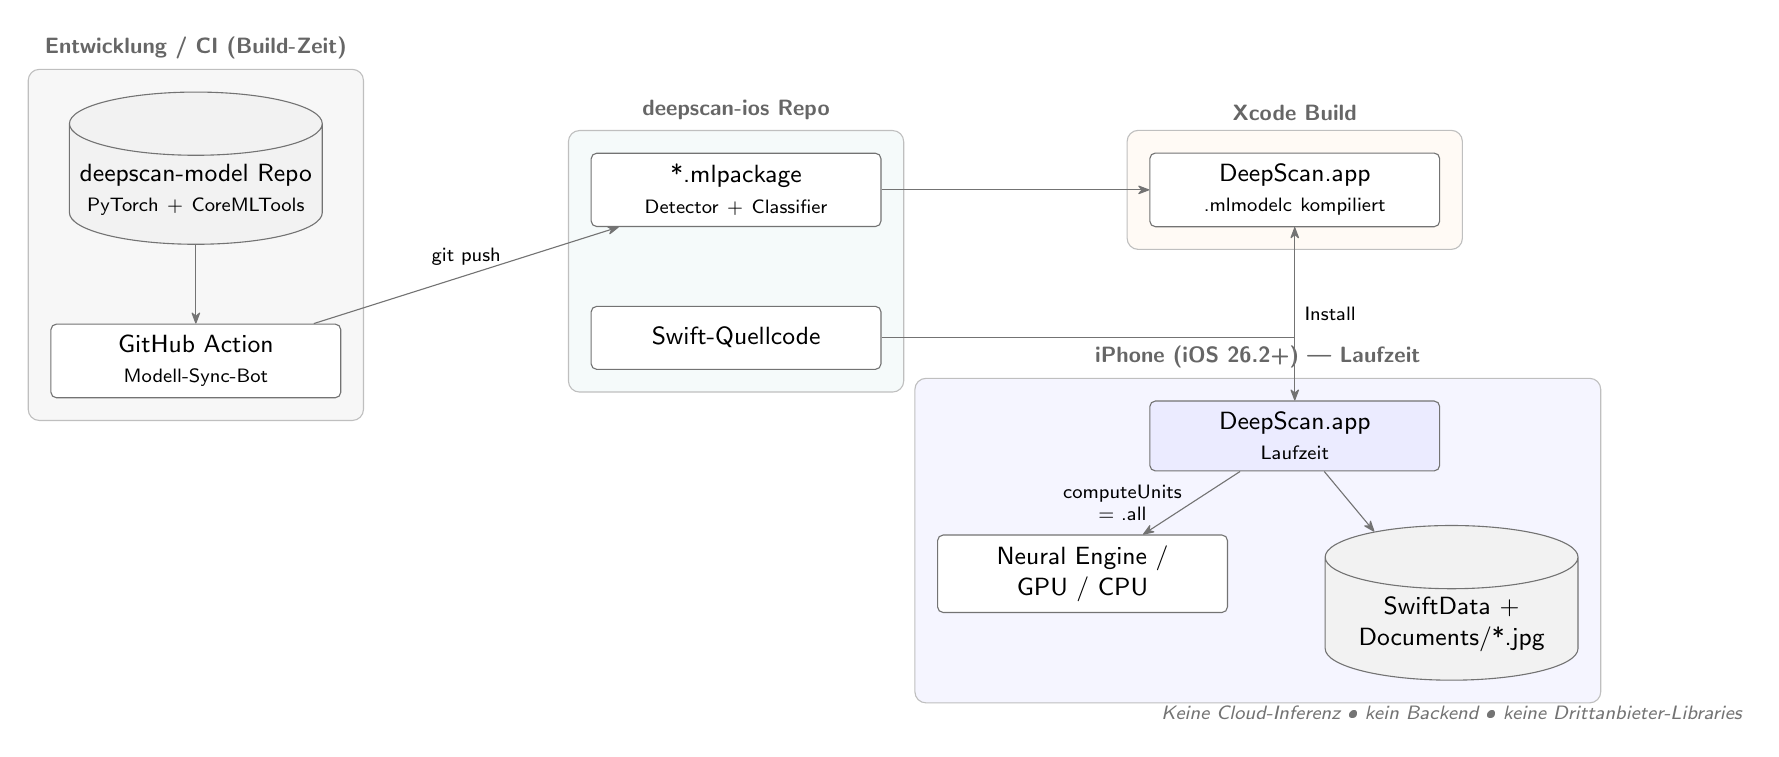
\begin{tikzpicture}[
    font=\small, >={Stealth[round]},
    box/.style={draw=black!55, rounded corners=2pt, fill=white, align=center,
                inner sep=4pt, minimum height=8mm, text width=34mm},
    db/.style={draw=black!55, cylinder, shape border rotate=90, aspect=0.25,
               fill=black!5, align=center, inner sep=3pt, text width=30mm, minimum height=12mm},
    grp/.style={draw=black!25, rounded corners=4pt, inner sep=8pt},
    lbl/.style={font=\footnotesize\bfseries, text=black!60},
    flow/.style={->, draw=black!55, font=\scriptsize},
]
% CI / dev
\node[db] (mrepo) {deepscan-model Repo\\\scriptsize PyTorch + CoreMLTools};
\node[box, below=10mm of mrepo] (gh) {GitHub Action\\\scriptsize Modell-Sync-Bot};
\draw[flow] (mrepo) -- (gh);

% iOS repo
\node[box, right=34mm of mrepo] (mlpkg) {*.mlpackage\\\scriptsize Detector + Classifier};
\node[box, below=10mm of mlpkg] (src) {Swift-Quellcode};
\draw[flow] (gh) -- (mlpkg) node[midway,above]{git push};

% Xcode
\node[box, right=34mm of mlpkg] (app) {DeepScan.app\\\scriptsize .mlmodelc kompiliert};
\draw[flow] (mlpkg) -- (app);
\draw[flow] (src) -| (app);

% Device
\node[box, below=22mm of app, fill=blue!8] (rt) {DeepScan.app\\\scriptsize Laufzeit};
\node[box, below left=8mm and -10mm of rt] (ane) {Neural Engine /\\GPU / CPU};
\node[db, below right=8mm and -10mm of rt] (store) {SwiftData +\\Documents/*.jpg};
\draw[flow] (app) -- (rt) node[midway,right]{Install};
\draw[flow] (rt) -- (ane) node[midway,left,align=center]{\scriptsize computeUnits\\\scriptsize = .all};
\draw[flow] (rt) -- (store);

\begin{scope}[on background layer]
    \node[grp, fill=black!3, fit=(mrepo)(gh), label={[lbl]north:Entwicklung / CI (Build-Zeit)}] {};
    \node[grp, fill=teal!4, fit=(mlpkg)(src), label={[lbl]north:deepscan-ios Repo}] {};
    \node[grp, fill=orange!4, fit=(app), label={[lbl]north:Xcode Build}] {};
    \node[grp, fill=blue!4, fit=(rt)(ane)(store), label={[lbl]north:iPhone (iOS 26.2+) — Laufzeit}] {};
\end{scope}
\node[align=center, font=\scriptsize\itshape, text=black!55, below=2mm of store]
    {Keine Cloud-Inferenz \textbullet\ kein Backend \textbullet\ keine Drittanbieter-Libraries};
\end{tikzpicture}
\end{document}
